\documentclass{report}

% Language setting
\usepackage[main=portuguese, english]{babel}
\usepackage{csquotes}

% Set page size and margins
\usepackage[a4paper,top=2cm,bottom=2cm,left=3cm,right=3cm,marginparwidth=1.5cm]{geometry}

% Useful packages
\usepackage{ulem}
\usepackage{parskip}
\usepackage{indentfirst}
\usepackage{setspace}
\usepackage{amsmath}
\usepackage{array}

\usepackage{graphicx}
\usepackage{xcolor}
\usepackage{colortbl}
\usepackage{subfigure}
\usepackage{titlesec}
\usepackage[colorlinks=false, allbordercolors={0 0 0}, pdfborderstyle={/S/U/W 0.25}]{hyperref}
\usepackage[hypcap=true]{caption}
\usepackage{enumitem}
\usepackage{soul}

\usepackage[siunitx]{circuitikz}

% Set section numbering from 1.1
\renewcommand{\thesection}{\arabic{section}.1}

\let\oldsection\section
\renewcommand\section{\clearpage\oldsection}

% Change section formatting
\titleformat{\section}
  {\fontsize{12}{15}\selectfont\bfseries}{\thesection}{1em}{}

% Configure indentations
\setlength{\parindent}{1.5cm}

\begin{document}

    \begin{titlepage}
        \centering
        
        \LARGE {Universidade Federal do Rio Grande do Sul \\ Escola de Engenharia}
    
        \begin{figure}[h!]
        \centering
        \subfigure
        {
\includegraphics[width=0.35\linewidth]{images/logos/UFRGS.png}}
        \hspace{1cm}
        \subfigure
        {
\includegraphics[width=0.3\linewidth]{images/logos/EE.png}}
        \end{figure}
    
        \LARGE {ENG10001 \\ Circuitos Elétricos I-C}
        
        \vfill
        {\noindent\hrulefill \\
        \bfseries \Huge{Trabalho Bônus 1} \\ \LARGE{Associação de Quadripolos} \\
        \noindent\hrulefill}
        
        \vfill
        {\LARGE Pedro Lubaszewski Lima (00341810) \\~\\ Turma A}
    
        \vfill
        {\LARGE 8 de dezembro de 2024}
        
    \end{titlepage}

        \renewcommand{\contentsname}{Sumário}
        \tableofcontents
        \clearpage
        \addtocontents{toc}{\protect\thispagestyle{empty}}

\section{Circuitos Sorteados}

Primeiramente, com o meu número de matrícula \textbf{0 0 3 4 1 8 1 0}, observa-se os seguintes dígitos sorteadores:

\begin{itemize}
  \item $ N_1 = 3$;
  \item $ N_2 = 4$;
  \item $ N_3 = 1$;
  \item $ N_4 = 8$;
  \item $ N_5 = 1$;
  \item $ N_6 = 0$.
\end{itemize}

A partir deles, sabe-se que os circuito a serem analisados são os seguintes:
\begin{figure}[h!]
    \centering
    \begin{circuitikz}
        \draw
        (3,3) to[R, l=4<\ohm>] (0,3)
        to[american voltage source, l=12<\volt>] (0,0)
        to[R, l_=16<\ohm>] (3,0)
        to[R, l_=10<\ohm>, *-*] (3,3)
        to[R, l_=20<\ohm>] (6,3)
        (3,0) to[R, l_=5<\ohm>] (6,0)
        (6,0) to[american current source, l_=3<\ampere>, *-*] (6,3)
        (6,3) -- (8,3) (6,0) -- (8,0)
        (8,3) to[R, l=5<\ohm>, *-*] (8,0)
        (8,3) -- (10,3) node[ocirc=](A){} node[right]{A}
        (8,0) -- (10,0) node[ocirc](B){} node[right]{B}

    ; \end{circuitikz}
    \caption{\label{ckt:input_1} Circuito de Entrada 2}
\end{figure}

\section{Circuito Equivalente de Thevénin da Entrada}

\section{Análise da Associação de Quadripolos}

\subsection{Representação dos Circuitos}

\subsection{Parâmetros do Quadripolo \texttt{Q1}}

\subsection{Parâmetros do Quadripolo \texttt{Q2}}

\subsection{União dos Quadripolos}

\section{Circuito Equivalente de Norton da Saída}

\section{Ganho de Tensão da Saída \texorpdfstring{\texttt{V\textsubscript{2}/V\textsubscript{1}}}{V2/V1}}

\section{Exemplos}

\begin{figure}[h!]
  \centering
  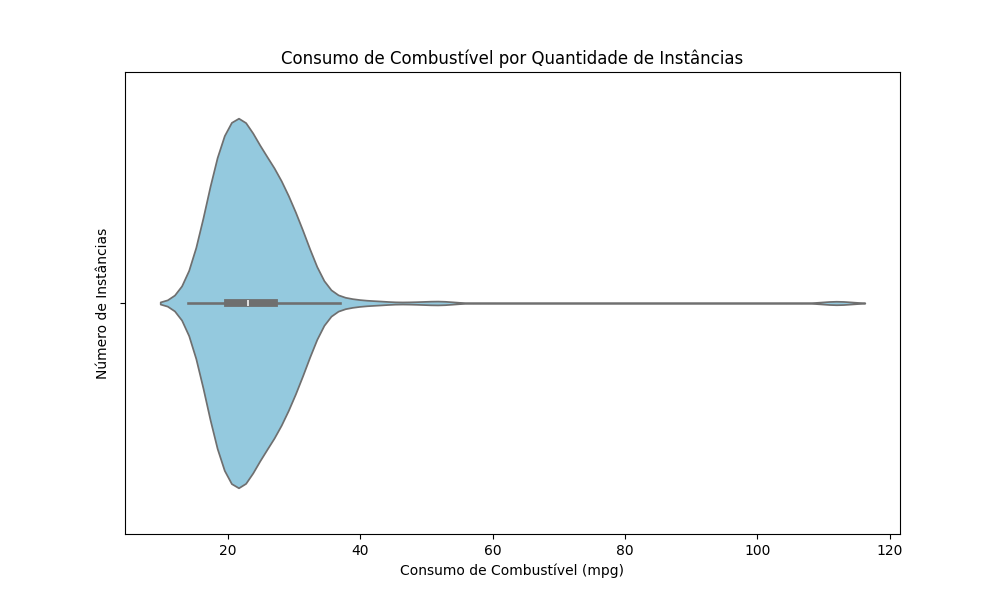
\includegraphics[width=.85\linewidth]{images/plots/violin_plots/pure_combination_mpg.png}
  \caption{\label{img:combination_dist} \textit{Violin Plot} de Consumo Médio}
\end{figure}

\begin{table}[h!]
  \centering
  \begin{tabular}{| c | c | c |}
      \hline
      \rowcolor{lightgray}
      \textbf{Modelo} & \textbf{Média dos MSE} & \textbf{Desvio Padrão dos MSE} \\
      \hline
      kNN & 5,4293 & 2,3616 \\
      \hline
      \textit{Random Forest} & 1,9517 & 1,1847 \\
      \hline
      Regressão Linear & 1,6631 & 0,9758 \\
      \hline
      Redes Neurais & 1,8377 & 1,0418 \\
      \hline
      SVM & 3,3739 & 1,3368 \\
      \hline
  \end{tabular}
  \caption{\label{table:model_summary} Médias e Desvios Padrões dos MSE}
\end{table}

\end{document}